\documentclass[11pt,a4paper]{article}
\usepackage[UTF8]{ctex}
\usepackage[a4paper,left=25mm,right=25mm,top=22mm,bottom=22mm]{geometry}
\usepackage{fontspec,xeCJK,graphicx,amsmath,amssymb}
\usepackage[hidelinks]{hyperref}
\setmainfont{Times New Roman}
\setCJKmainfont{SimSun}[BoldFont=SimHei]
\setCJKsansfont{SimHei}
\setlength{\parindent}{2em}
\setlength{\parskip}{3pt}
\linespread{1.18}
\emergencystretch=1em
\widowpenalty=10000
\clubpenalty=10000
\setlength{\abovecaptionskip}{5pt}
\graphicspath{{../figures/eda-v2/}}
\makeatletter
\newenvironment{inlinefigure}{\par\addvspace{10pt}\noindent\begin{minipage}{\linewidth}\def\@captype{figure}\centering}{\end{minipage}\par\addvspace{10pt}}
\makeatother
\pagestyle{plain}
\begin{document}

\section*{7 数据预处理与探索性分析}

\subsection*{7.1 数据预处理}

本文使用题目附件中的代表日供需、全年实际负载与光伏、光伏预报及电价数据。预处理时，统一日期和时间的写法，将同一时刻的负载、光伏和电价对应起来，并保留每次发布的光伏预报。整理后的数值与原表逐项核对一致，没有改变原始数值。以下日均、月均功率均由相应采样值取平均得到。

经过整理与分析，我们有以下发现。

\subsection*{7.2 光伏富余与用电需求在时间上错开}

微网面临的首要问题是发电与用电在时间上的不一致。如图\ref{fig:reference}所示，光伏在白天逐渐增强，午间可以覆盖负载并产生富余；傍晚光伏回落后，小区仍有较高的用电需求。电价在晚间也处于较高水平，使这一阶段补充供电的成本更高。图中的负载与光伏功率差直观地反映了这种变化：午间出现富余，傍晚又需要外网或电池补充。

\begin{inlinefigure}
  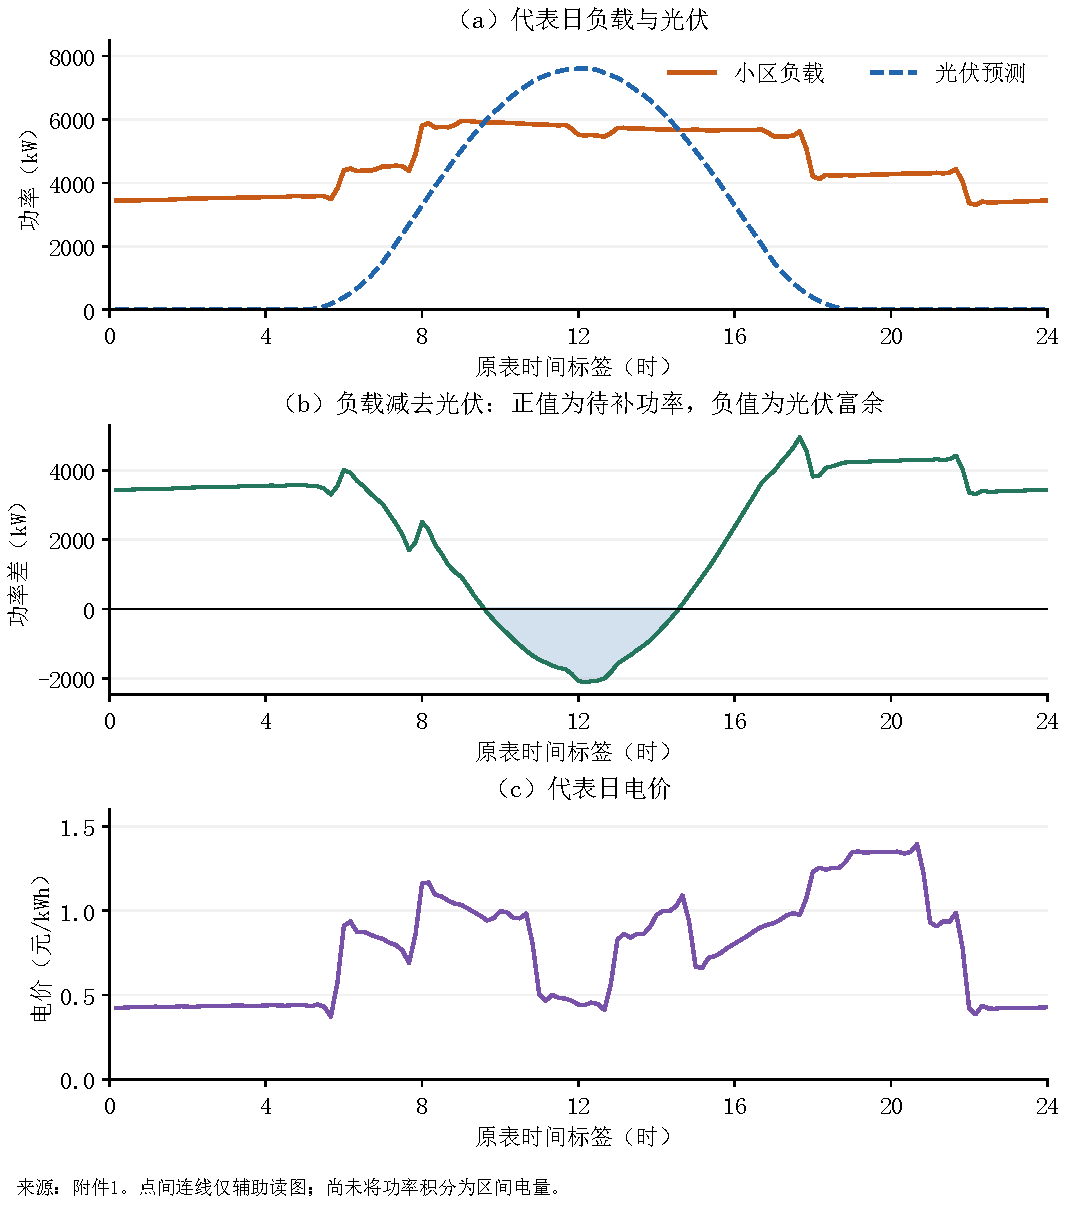
\includegraphics[width=0.82\linewidth]{01_reference_day.pdf}
  \caption{代表日供需与电价的时间错配}
  \label{fig:reference}
\end{inlinefigure}

代表日午间的最大富余功率约为2100 kW，而傍晚需要补充的功率最高接近5000 kW。这说明，白天发电充足并不能直接解决晚间供电问题。电池可以把部分富余电量留到以后使用，但必须先有空间接收，并能在需要时及时放出。因此，购电安排既与当时的供需差额有关，也与之前储存了多少电、之后还要应对多大需求有关。

这种时间错配并非仅出现在代表日：全年有330天出现过光伏超过负载的记录，接收和利用午间富余是经常需要面对的情景。不过，附件1接近全年各时刻的平均供需形状，具体日期仍会出现更高的负载峰值或不同程度的光伏富余。代表日能够说明储能转移电量的基本作用，却不足以代表每一天的运行压力。富余电量最终能利用多少，还取决于当时的电池状态，不能由富余出现的次数直接判断。

\subsection*{7.3 用电高峰与供需缺口的季节变化不同步}

从图\ref{fig:annual}可以看到，负载与光伏都有明显的年内变化，但二者并不同步。夏季负载较高，同时也有较多光伏补充；进入冬季后，负载虽低于夏季高峰，光伏却明显减少。这使微网对外网补充的需求，不能仅按负载高低来判断。图中的逐日曲线还呈现出月均水平周围的持续起伏，说明季节变化与日际差异同时存在。

\begin{inlinefigure}
  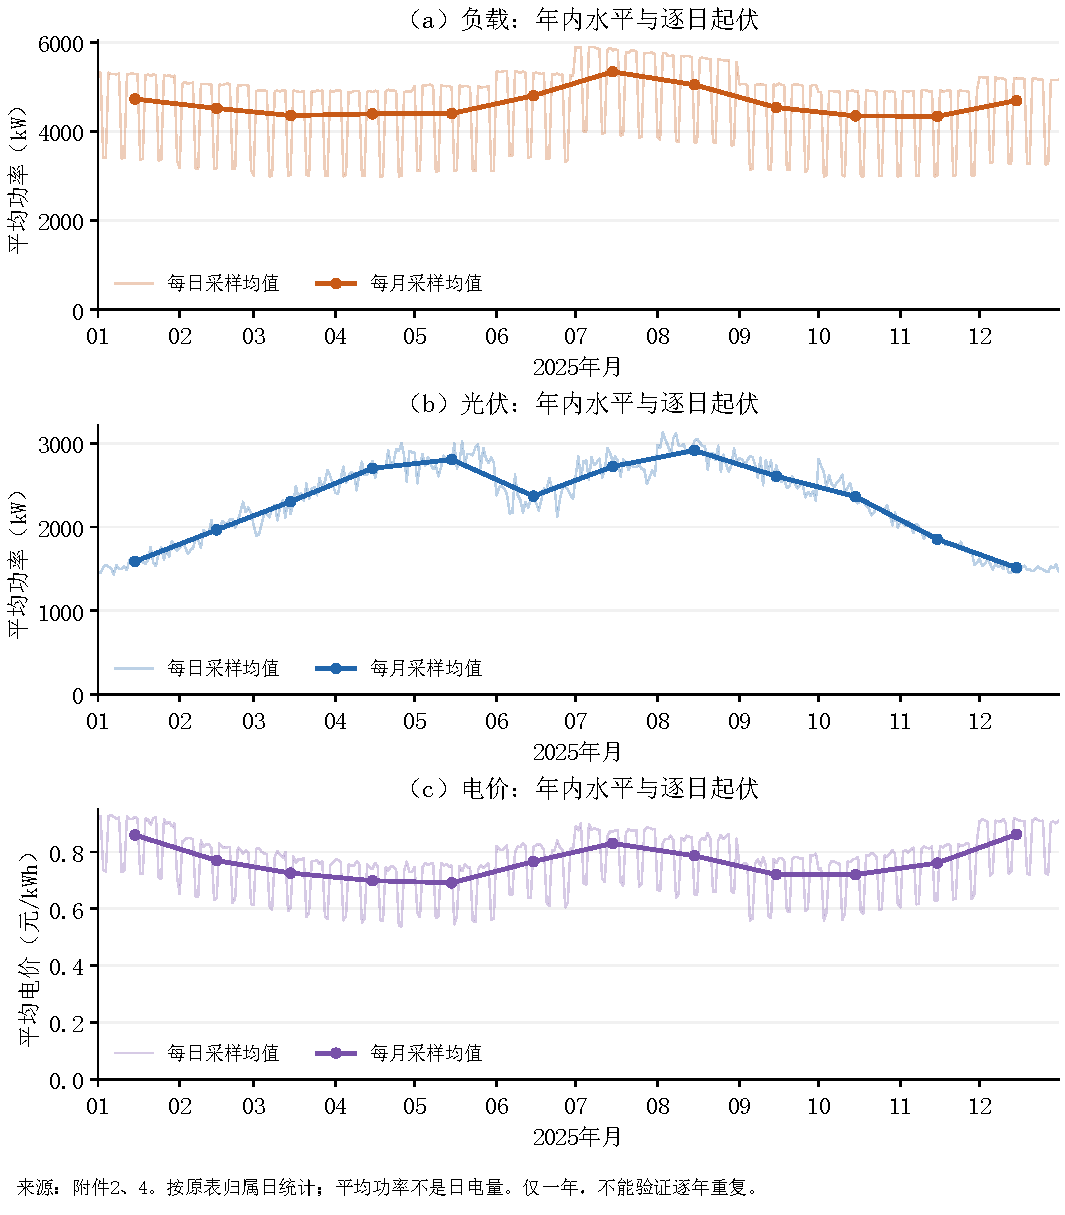
\includegraphics[width=0.82\linewidth]{02_year_and_month.pdf}
  \caption{负载、光伏与电价的年内变化}
  \label{fig:annual}
\end{inlinefigure}

以冬春差异为例，12月平均负载减去光伏后的功率差约为3180 kW，而5月约为1600 kW，前者接近后者的两倍。冬季供需差额较大，并不意味着用电一定更多，而是本地光伏能够承担的部分更少。对储能而言，这也意味着不同季节可供储存的光伏余量和随后需要补充的电力并不相同，全年照用同一套购电、充放电安排，难以适应这种变化。

年内变化也不是平滑的增减。例如，光伏月均功率在6月出现回落，低于相邻月份。附件没有对应天气资料，因此这里只将其视为实际数据中的变化，不推断具体气象原因。现有记录支持2025年存在明显季节差异，是否逐年以同样方式重复，还需要其他年份的数据验证。

\subsection*{7.4 负载有周重复，电价仍存在跨日波动}

负载除了随季节变化，还表现出清楚的星期差异。按原始日期分组，周五和周六的平均负载比其余五天低约36.8\%，且各月均能观察到这一特点，见图\ref{fig:prices}。这意味着，相邻两天虽然在时间上更近，用电水平却未必更接近；参考历史负载时，同一星期位置的记录也可能提供有用信息。该分组来自附件日期，不据此推断居民的具体作息制度。

\begin{inlinefigure}
  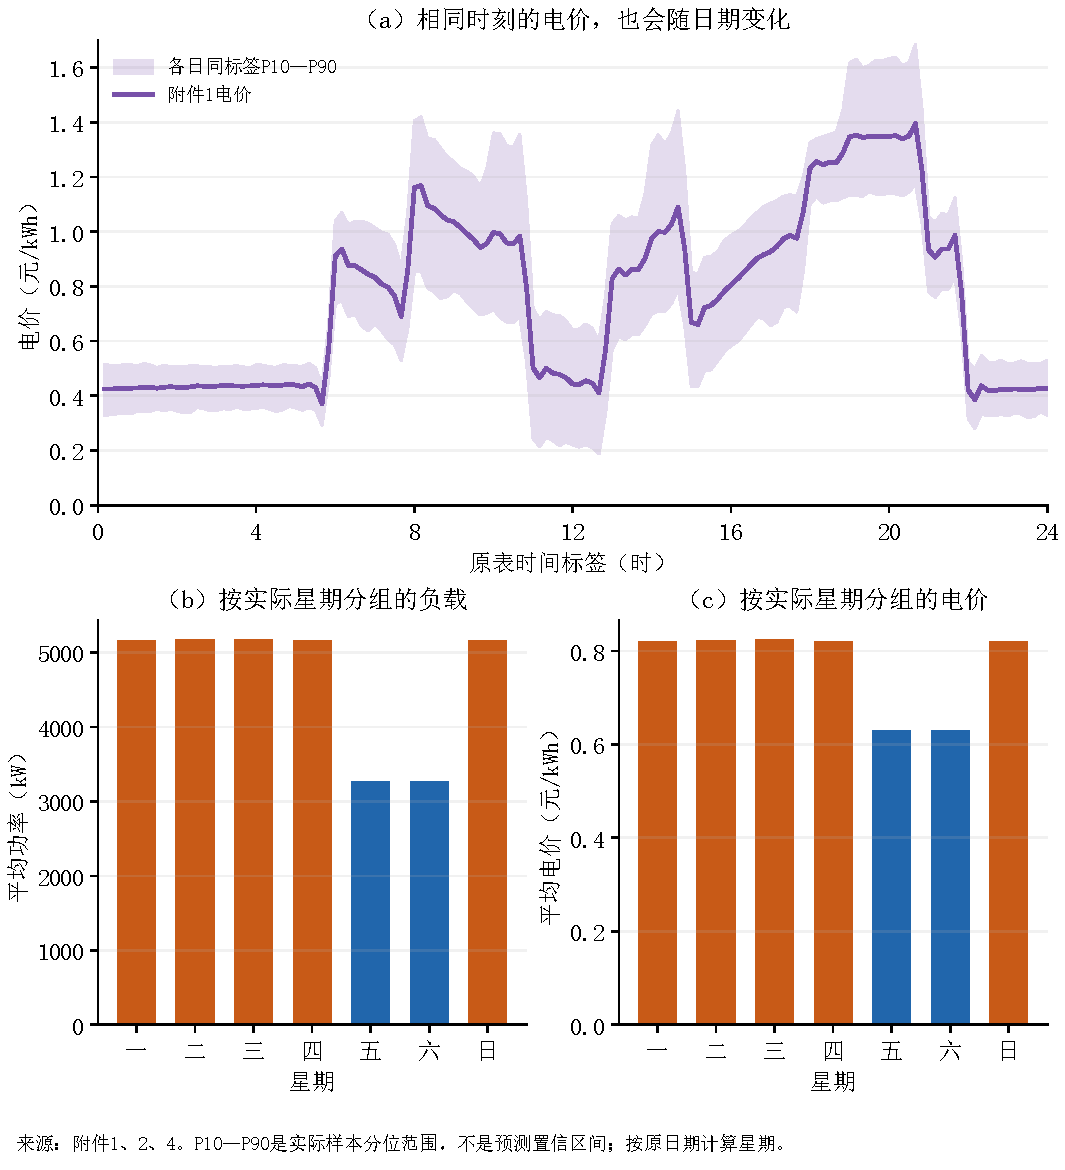
\includegraphics[width=0.78\linewidth]{06_prices_and_weekdays.pdf}
  \caption{不同星期的用电差异与同一时刻的电价波动}
  \label{fig:prices}
\end{inlinefigure}

将序列与一周前的数值比较，并扣除各月相同时刻的平均轮廓后，负载和电价仍保持较强的相关性，而光伏的一周相关性已接近零。光伏原先较高的相似程度，主要来自白天发电、夜间接近零的共同形状。因此，这几类数据不能仅因都呈现重复起伏，就被视为具有相同的周规律；历史信息的参考方式需要适应各自的变化特点。

电价还存在同一时刻、不同日期之间的差异。图\ref{fig:prices}中的阴影给出全年各日同一时刻价格的第10至第90百分位范围，其宽度反映出固定日内曲线没有呈现的波动。历史上较便宜的时段仍可作为参考，但并不保证下一天也同样便宜。按第四问采用的信息条件，未来真实价格尚不可知，提前充电的收益也就存在不确定性：低价购电能否弥补充放电损耗，取决于之后实际遇到的价格和用电需求。

\subsection*{7.5 光伏预报更新的改善与局限}

附件3的预报整体呈现出提前越久、误差越大的特点，如图\ref{fig:forecast}所示。比较时，将预报与同一目标整点的实测值对应，以两者绝对差的平均值衡量偏差；年末超出实测覆盖范围的36条预报不参与误差计算。图中还区分了全部记录与实际有光伏的记录：夜间接近零的数值会降低总体平均误差，因此仅看总体结果，容易忽略实际发电时更大的供需偏差。

\begin{inlinefigure}
  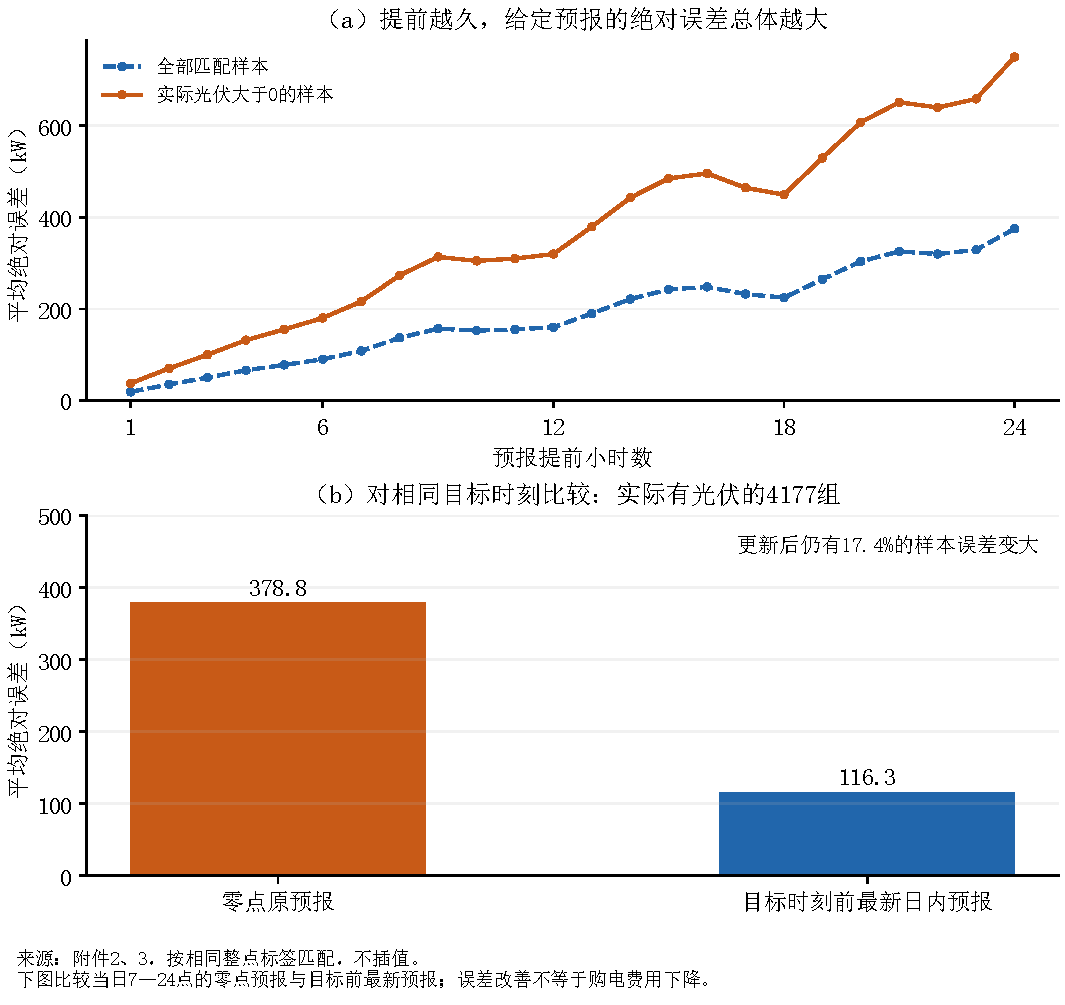
\includegraphics[width=0.78\linewidth]{07_forecast_accuracy.pdf}
  \caption{预报提前量与日内更新对光伏预报误差的影响}
  \label{fig:forecast}
\end{inlinefigure}

为直接观察更新的作用，对每天7点至24点的同一目标时刻，比较零点预报与目标发生前已经发布的最新预报。在实测光伏大于零的4177组配对中，平均绝对误差由约379 kW降至116 kW，减少约69\%。这说明，日内更新确实改善了这组数据中对未来光伏的判断。不过，仍有约17.4\%的配对在更新后误差增大，新预报并非每次都更准确。这里按实测值分组是为了观察发电时的误差，制定计划时并不能提前知道实际光伏。

更准确的信息为调整购电提供了依据，但其经济作用还取决于电池和合同。如果原计划的偏差可以由电池吸收，修改购电量未必划算；如果预计偏差较大、储能又缺少调节余地，提前调整才可能减少昂贵的紧急补购。预报更新的价值取决于它是否改变了实际需要的购电量，以及节省的补购费用能否抵偿调整费用，不能直接用平均误差的降幅代表节费比例。

\end{document}
